\documentclass{minimal}

\usepackage[paperwidth=20cm,paperheight=28cm,margin=1cm]{geometry}

\usepackage[utf8]{inputenc}
\usepackage[T1]{fontenc}
\usepackage[american]{babel}

\usepackage{amsmath}
\usepackage{tikz}
\usetikzlibrary{automata,arrows,positioning}

\newcommand{\anobs}[1][\mathtt{k}]{\mathcal{O}_{#1}}
\newcommand{\baseobs}{\anobs[\mkern-1mu\mathit{Base}]}
\newcommand{\hpobs}{\anobs[\mkern-1mu\mathit{HP}]}
\newcommand{\translab}[2]{\ensuremath{#1,\,#2}}
\newcommand{\translabbr}[2]{\ensuremath{#1},\\\ensuremath{#2}}
\newcommand{\anadr}{a}
\newcommand{\athread}{t}
\newcommand{\threadvar}{z_{t}}
\newcommand{\adrvar}{z_a}
\newcommand{\evt}[2]{#1(#2)}
\newcommand{\enter}{\mathtt{enter}}
\newcommand{\enterof}[1]{\enter\:#1}
\newcommand{\exit}{\mathtt{exit}}
\newcommand{\exitof}[1]{\exit\:#1}
\newcommand{\free}{\mathtt{free}}
\newcommand{\freeof}[1]{\free(#1)}
\newcommand{\retire}{\mathtt{retire}}
\newcommand{\guard}[1][]{\mathtt{protect}_{\mathtt{#1}}}
\newcommand{\guardof}[2][]{\guard[#1](#2)}

\newcounter{ObserverStateCounter}
\newcommand{\mkstatename}[1]{\stepcounter{ObserverStateCounter}${\arabic{ObserverStateCounter}}$}


\begin{document}
	\centering

	The SMR automaton specifying Hazard Pointers (HP) is defined by $\baseobs\times\hpobs$.
	\vspace{1cm}

	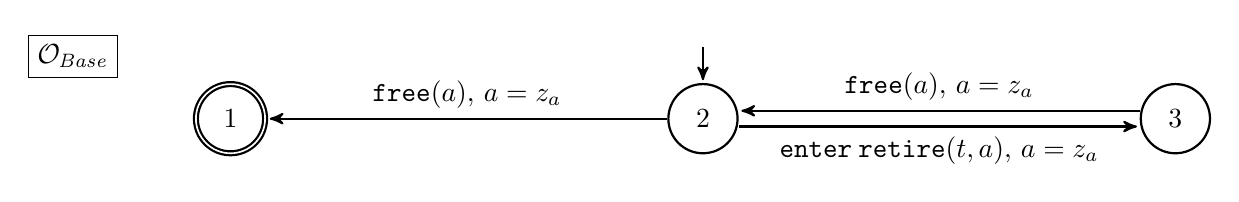
\begin{tikzpicture}[->,>=stealth',shorten >=1pt,auto,node distance=6cm,thick,initial text={}]
		\node [xshift=-2.0cm,yshift=.79cm,draw,thin] {$\baseobs$};
		\node[accepting,state]      (C)               {\mkstatename{obs:base:final}};
		\node[initial above, state] (A) [right of=C]  {\mkstatename{obs:base:init}};
		\node[state]                (B) [right of=A]  {\mkstatename{obs:base:retired}};
		\path
			([yshift=1mm]B.west) edge node [above]{\translab{\freeof{\anadr}}{\anadr=\adrvar}} ([yshift=1mm]A.east)
			([yshift=-1mm]A.east) edge node [below]{\translab{\evt{\enterof{\retire}}{\athread,\anadr}}{\anadr=\adrvar}} ([yshift=-1mm]B.west)
			(A) edge node [above]{\translab{\freeof{\anadr}}{\anadr=\adrvar}} (C)
			;
	\end{tikzpicture}
	\vspace{1cm}

	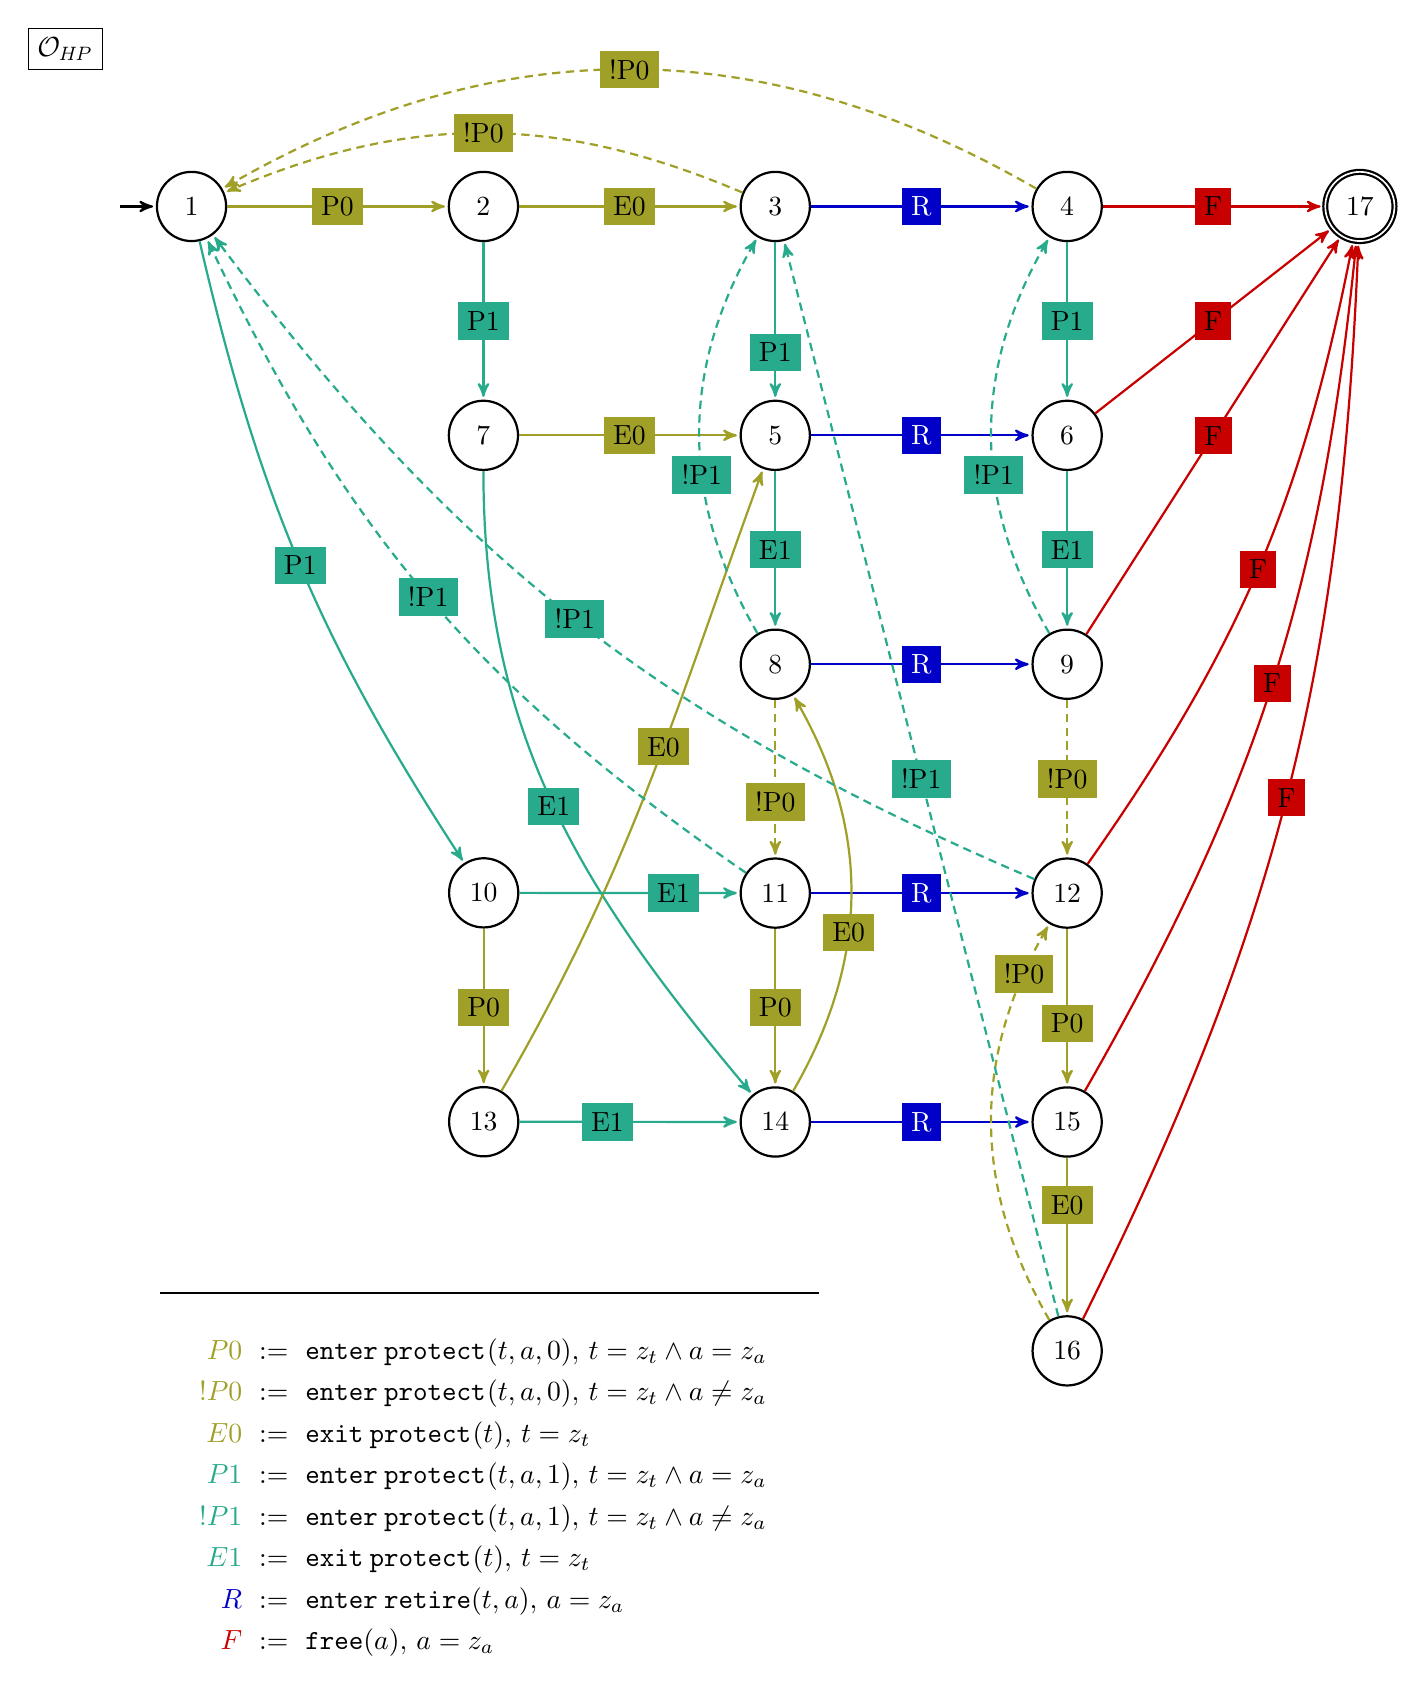
\begin{tikzpicture}[->,>=stealth',shorten >=1pt,auto,node distance=2cm and 2.8cm,thick,initial text={}]
		% name
		\node [xshift=-1.6cm,yshift=2cm,draw,thin] {$\hpobs$};

		% states
		\node[initial,state] (S1) {\mkstatename{obs:hp:s1}};
		\node[state] (S2) [right=of S1] {\mkstatename{obs:hp:s2}};
		\node[state] (S3) [right=of S2] {\mkstatename{obs:hp:s3}};
		\node[state] (S4) [right=of S3] {\mkstatename{obs:hp:s4}};
		\node[state] (S5) [below=of S3] {\mkstatename{obs:hp:s5}};
		\node[state] (S6) [below=of S4] {\mkstatename{obs:hp:s6}};
		  \node[state] (S16) [below=of S2] {\mkstatename{obs:hp:s16}};
		\node[state] (S7) [below=of S5] {\mkstatename{obs:hp:s7}};
		\node[state] (S8) [below=of S6] {\mkstatename{obs:hp:s8}};
		\coordinate [below=of S7,yshift=-4.5mm,xshift=-4.5mm] (XX) {};
		\node[state] (S9) [left=of XX] {\mkstatename{obs:hp:s9}};
		\node[state] (S10) [below=of S7] {\mkstatename{obs:hp:s10}}; % name problem
		\node[state] (S11) [below=of S8] {\mkstatename{obs:hp:s11}};
		  \node[state] (S17) [below=of S9] {\mkstatename{obs:hp:s17}};
		\node[state] (S12) [below=of S10] {\mkstatename{obs:hp:s12}};
		\node[state] (S13) [below=of S11] {\mkstatename{obs:hp:s13}};
		% \node[state] (S14) [below=of S12] {\mkstatename{obs:hp:s14}};
		\node[state] (S15) [below=of S13] {\mkstatename{obs:hp:s15}};
		\node[accepting,state,double=white] (SF) [right=of S4] {\mkstatename{obs:hp:sf}};

		% shortcuts
		\newcommand{\EnterA}{P0}
		\newcommand{\EnterB}{P1}
		\newcommand{\EnterAo}{!P0}
		\newcommand{\EnterBo}{!P1}
		\newcommand{\ExitA}{E0}
		\newcommand{\ExitB}{E1}
		\newcommand{\Retire}{R}
		\newcommand{\Free}{F}

		\definecolor{colorEnterA}{RGB} {160,160,40}
		\definecolor{colorEnterAo}{RGB} {160,160,40}
		\definecolor{colorExitA}{RGB} {160,160,40}
		\definecolor{colorEnterB}{RGB} {40,170,140}
		\definecolor{colorEnterBo}{RGB} {40,170,140}
		\definecolor{colorExitB}{RGB} {40,170,140}
		\definecolor{colorRetire}{RGB} {0,0,200}
		\definecolor{colorFree}{RGB} {200,0,0}

		% trans
		\draw[colorEnterB] (S2) edge node[anchor=center,fill=colorEnterB,text=black] {\EnterB} (S16);
		\draw[colorExitA] (S16) edge node[anchor=center,fill=colorExitA,text=black] {\ExitA} (S5);
		\draw[colorExitB] (S16) edge[out=270,in=130] node[anchor=center,fill=colorExitB,text=black] {\ExitB} (S12);
		  % \draw[colorEnterAo] (S16) edge[out=265,in=95] node[anchor=center,fill=colorEnterAo,text=black,pos=.7] {\EnterAo} (S9);

		\draw[colorEnterA] (S9) edge node[anchor=center,fill=colorEnterA,text=black] {\EnterA} (S17);
		\draw[colorExitB] (S17) edge node[anchor=center,fill=colorExitB,text=black,pos=.4] {\ExitB} (S12);
		\draw[colorExitA] (S17) edge[out=60,in=250] node[anchor=center,fill=colorExitA,text=black,pos=.57] {\ExitA} (S5);

		% transitions
		\draw[colorEnterA] (S1) edge node[anchor=center,fill=colorEnterA,text=black] {\EnterA} (S2);
		\draw[colorExitA] (S2) edge node[anchor=center,fill=colorExitA,text=black] {\ExitA} (S3);
		\draw[colorRetire] (S3) edge node[anchor=center,fill=colorRetire,text=white] {\Retire} (S4);
		\draw[colorFree] (S4) edge node[anchor=center,fill=colorFree,text=black] {\Free} (SF);
		\draw[colorEnterB] (S3) edge node[anchor=center,fill=colorEnterB,text=black,pos=.7] {\EnterB} (S5);
		\draw[colorEnterB] (S4) edge node[anchor=center,fill=colorEnterB,text=black] {\EnterB} (S6);
		\draw[colorExitB] (S5) edge node[anchor=center,fill=colorExitB,text=black] {\ExitB} (S7);
		\draw[colorExitB] (S6) edge node[anchor=center,fill=colorExitB,text=black] {\ExitB} (S8);
		\draw[colorRetire] (S5) edge node[anchor=center,fill=colorRetire,text=white] {\Retire} (S6);
		\draw[colorRetire] (S7) edge node[anchor=center,fill=colorRetire,text=white] {\Retire} (S8);
		\draw[colorFree] (S6) edge node[anchor=center,fill=colorFree,text=black] {\Free} (SF);
		\draw[colorFree] (S8) edge node[anchor=center,fill=colorFree,text=black] {\Free} (SF);

		\draw[colorEnterAo,densely dashed] (S3) edge[bend right=23,above right] node[anchor=center,fill=colorEnterAo,text=black] {\EnterAo} (S1);
		\draw[colorEnterAo,densely dashed] (S4) edge[bend right,above right] node[anchor=center,fill=colorEnterAo,text=black] {\EnterAo} (S1);
		\draw[colorEnterAo,densely dashed] (S7) edge node[anchor=center,fill=colorEnterAo,text=black,pos=.65] {\EnterAo} (S10);
		\draw[colorEnterAo,densely dashed] (S8) edge node[anchor=center,fill=colorEnterAo,text=black] {\EnterAo} (S11);
		\draw[colorEnterBo,densely dashed] (S7) edge[bend left] node[anchor=center,fill=colorEnterBo,text=black,pos=.4] {\EnterBo} (S3); % label
		\draw[colorEnterBo,densely dashed] (S8) edge[bend left] node[anchor=center,fill=colorEnterBo,text=black,pos=.4] {\EnterBo} (S4); % label

		\draw[colorEnterB] (S1) edge[bend right=10] node[anchor=center,fill=colorEnterB,text=black] {\EnterB} (S9);
		\draw[colorExitB] (S9) edge node[anchor=center,fill=colorExitB,text=black,pos=.7] {\ExitB} (S10);
		\draw[colorRetire] (S10) edge node[anchor=center,fill=colorRetire,text=white] {\Retire} (S11);
		\draw[colorRetire] (S12) edge node[anchor=center,fill=colorRetire,text=white] {\Retire} (S13);
		% \draw[colorRetire] (S14) edge node[anchor=center,fill=colorRetire,text=white] {\Retire} (S15);
		\draw[colorEnterA] (S10) edge node[anchor=center,fill=colorEnterA,text=black] {\EnterA} (S12);
		\draw[colorEnterA] (S11) edge node[anchor=center,fill=colorEnterA,text=black,pos=.6] {\EnterA} (S13);
		\draw[colorExitA] (S12) edge[bend right=30,pos=.4] node[anchor=center,fill=colorExitA,text=black] {\ExitA} (S7); % (S14);
		\draw[colorExitA] (S13) edge node[anchor=center,fill=colorExitA,text=black,pos=.3] {\ExitA} (S15);
		\draw[colorFree] (S11) edge[bend right=12] node[anchor=center,fill=colorFree,text=black] {\Free} (SF);
		\draw[colorFree] (S13) edge[bend right=12] node[anchor=center,fill=colorFree,text=black] {\Free} (SF);
		\draw[colorFree] (S15) edge[bend right=12] node[anchor=center,fill=colorFree,text=black] {\Free} (SF);

		\draw[colorEnterBo,densely dashed] (S10) edge[bend left=15] node[anchor=center,fill=colorEnterBo,text=black] {\EnterBo} (S1); % label
		\draw[colorEnterBo,densely dashed] (S11) edge[bend left=15] node[anchor=center,fill=colorEnterBo,text=black] {\EnterBo} (S1); % label
		% \draw[colorEnterAo,densely dashed] (S14) edge[bend left] node[anchor=center,fill=colorEnterAo,text=black,pos=.6] {\EnterAo} (S10);
		\draw[colorEnterAo,densely dashed] (S15) edge[bend left] node[anchor=center,fill=colorEnterAo,text=black,pos=.875] {\EnterAo} (S11); % label
		% \draw[colorEnterBo,densely dashed] (S14) edge[bend left] node[anchor=center,fill=colorEnterBo,text=black,pos=.3] {\EnterBo} (S3); % label
		\draw[colorEnterBo,densely dashed] (S15) edge node[anchor=center,fill=colorEnterBo,text=black] {\EnterBo} (S3); % label


		% key
		\draw[-,line width=1pt] (-0.4,-13.8) -- (8,-13.8);
		\node [xshift=3.7cm,yshift=-16.4cm] {
			\(\begin{aligned}
				\color{colorEnterA}{\EnterA} ~&:=~ \translab{\evt{\enterof{\guard}}{\athread,\anadr,0}}{\athread=\threadvar\wedge\anadr=\adrvar}
				\\
				\color{colorEnterAo}{\EnterAo} ~&:=~ \translab{\evt{\enterof{\guard}}{\athread,\anadr,0}}{\athread=\threadvar\wedge\anadr\neq\adrvar}
				\\
				\color{colorExitA}{\ExitA} ~&:=~ \translab{\evt{\exitof{\guard}}{\athread}}{\athread=\threadvar}
				\\
				\color{colorEnterB}{\EnterB} ~&:=~ \translab{\evt{\enterof{\guard}}{\athread,\anadr,1}}{\athread=\threadvar\wedge\anadr=\adrvar}
				\\
				\color{colorEnterBo}{\EnterBo} ~&:=~ \translab{\evt{\enterof{\guard}}{\athread,\anadr,1}}{\athread=\threadvar\wedge\anadr\neq\adrvar}
				\\
				\color{colorExitB}{\ExitB} ~&:=~ \translab{\evt{\exitof{\guard}}{\athread}}{\athread=\threadvar}
				\\
				\color{colorRetire}{\Retire} ~&:=~ \translab{\evt{\enterof{\retire}}{\athread,\anadr}}{\anadr=\adrvar}
				\\
				\color{colorFree}{\Free} ~&:=~ \translab{\freeof{\anadr}}{\anadr=\adrvar}
			\end{aligned}\)
		};
	\end{tikzpicture}

\end{document}
